\documentclass{beamer}
\usetheme{CambridgeUS}
\usepackage[utf8]{inputenc}
 
\usepackage{tfrupee}
\usepackage{enumitem}
\usepackage{amsmath}
\usepackage{amssymb}
\usepackage{graphicx}
\usepackage{mathtools}
\providecommand{\sbrak}[1]{\ensuremath{{}\left[#1\right]}}
\providecommand{\lsbrak}[1]{\ensuremath{{}\left[#1\right.}}
\providecommand{\rsbrak}[1]{\ensuremath{{}\left.#1\right]}}
\providecommand{\brak}[1]{\ensuremath{\left(#1\right)}}
\providecommand{\lbrak}[1]{\ensuremath{\left(#1\right.}}
\providecommand{\rbrak}[1]{\ensuremath{\left.#1\right)}}
\providecommand{\cbrak}[1]{\ensuremath{\left\{#1\right\}}}
\providecommand{\lcbrak}[1]{\ensuremath{\left\{#1\right.}}
\providecommand{\rcbrak}[1]{\ensuremath{\left.#1\right\}}}

\newcommand{\myvec}[1]{\ensuremath{\begin{pmatrix}#1\end{pmatrix}}}
\let\vec\mathbf

\title{Assignment 6}
\author{\textbf{Himanshu Kumar Gupta (AI21BTECH11012)}}
\date {May 2022}

\begin{document}
\begin{frame}
    \maketitle
\end{frame}

\begin{frame}{Contents}
\tableofcontents
\end{frame}
\section{Question}

\begin{frame}{Ex. 4.24 , chapter 4 , Papoulis}
    \textbf{A fair coin is tossed n times. Find n such that the probability that the number of heads is between 0.49n and 0.52n is at least 0.9.}
\end{frame}



\section{Solution}
\begin{frame}{Solution}
    


Since the coin is fair.
So,
\begin{align}
  p=q=0.5  
\end{align}


No. of heads would be in between .49n and .52n. 
So,
\begin{align}
    k_1=.49n          \\
k_2=.52n
\end{align}
\end{frame}
\begin{frame}
    


Now,
\begin{align}
    \frac{k_2-pn}{\sqrt{pqn}}&=\frac{.52n-.5n}{\sqrt{.5\times.5n}}  \nonumber \\
    &=\frac{.02n}{.5\sqrt{n}}           \nonumber \\
    &=.04\sqrt{n}
\end{align}

\begin{align}
     \frac{k_1-pn}{\sqrt{pqn}}&=\frac{.49n-.5n}{\sqrt{.5\times.5n}}  \nonumber \\
    &=\frac{-.01n}{.5\sqrt{n}}           \nonumber \\
    &=-.02\sqrt{n}
\end{align}
\end{frame}
\begin{frame}
So,
\begin{align}
    P(.49n \leq k \leq .52n)&=G(\frac{k_2-pn}{\sqrt{pqn}})-G(\frac{k_1-pn}{\sqrt{pqn}}) \geq .9  \nonumber\\
    &=G(.04\sqrt{n})-G(-.02\sqrt{n}) \geq .9    \nonumber  \\
    &=G(.04\sqrt{n})+G(.02\sqrt{n})-1  \geq .9    \nonumber \\
    &=G(.04\sqrt{n})+G(.02\sqrt{n})  \geq 1.9    \nonumber   \\
\end{align}
using table,we get that
\begin{align}
    .02\sqrt{n}>1.3  \nonumber \\
\sqrt{n}>65    \nonumber        \\
n>65^2
\end{align}
\end{frame}
\begin{frame}
    \begin{figure}[htb!]
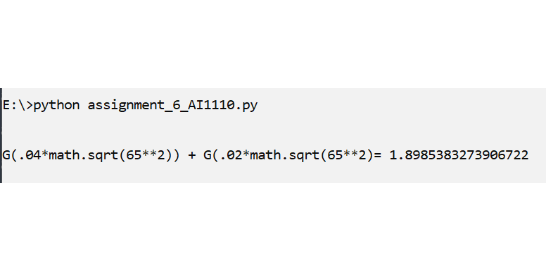
\includegraphics[width=12cm]{figures/assignment_6_output.png}
\caption{code output}
\end{figure}

\end{frame}
\begin{frame}
    \begin{figure}[htb!]

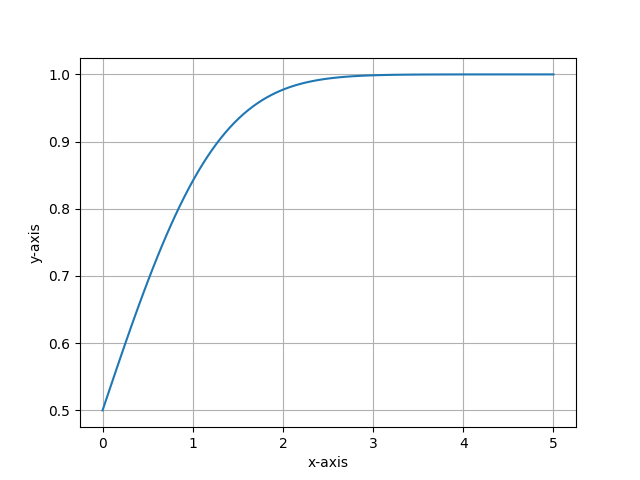
\includegraphics[width=10cm]{figures/G(x)_function.png}
\caption{G(x) function}
\end{figure}

\end{frame}


\end{document}